\documentclass[../thesis.tex]{subfiles}

\providecommand{\zcut}{\mathrm{z_{cut}}}


\setlength{\parskip}{0pt}
%%
%% End Preamble
%%
%% The fun begins:
\begin{document}
\section{The physics of elementary particles}
	Modern particle physics is, ultimately, the result of a confluence of an ancient problem and an ancient technique. The problem: how does nature work on the most fundamental level? The technique: to smash objects together and see what comes out. 

	Of course, thousands of years of scientific development have led us to a more nuanced and sophisticated understanding than, say, the early atomic theories of Democritus and Lucretius --- though echoes of these theories remain. We now understand\footnote{Or at least, believe to understand.} that almost all visible matter and almost all observed forces are, at root, manifestations of interactions between 17 fundamental particles (though there may yet be more). We conceive of these particles as excitations in fields which permeate space-time --- this conception is known as quantum field theory.\footnote{Space-time itself is a geometric entity --- we perceive this geometry as the force of gravity, acting on both human and cosmic scales --- described by the theory of General Relativity.}

	The goal of elementary particle physics\footnote{Also known simply as particle physics or high-energy physics.} is to understand these particles and fields at the deepest level.\footnote{Some particle theorists are also trying to unite quantum field theory with General Relativity. Whether they will ever succeed remains to be seen, but they do lots of pretty math.} We would like to lay a complete framework, understanding their nature and their interactions to such an extent that one could, in principle, derive from first principles an explanation for any observed physical phenomenon. The field is a long way from that goal, but much progress has been made over the past centuries. Let us begin by summarizing what we know so far.

\subsection{The Standard Model}
	\begin{figure}
	\begin{centering}
		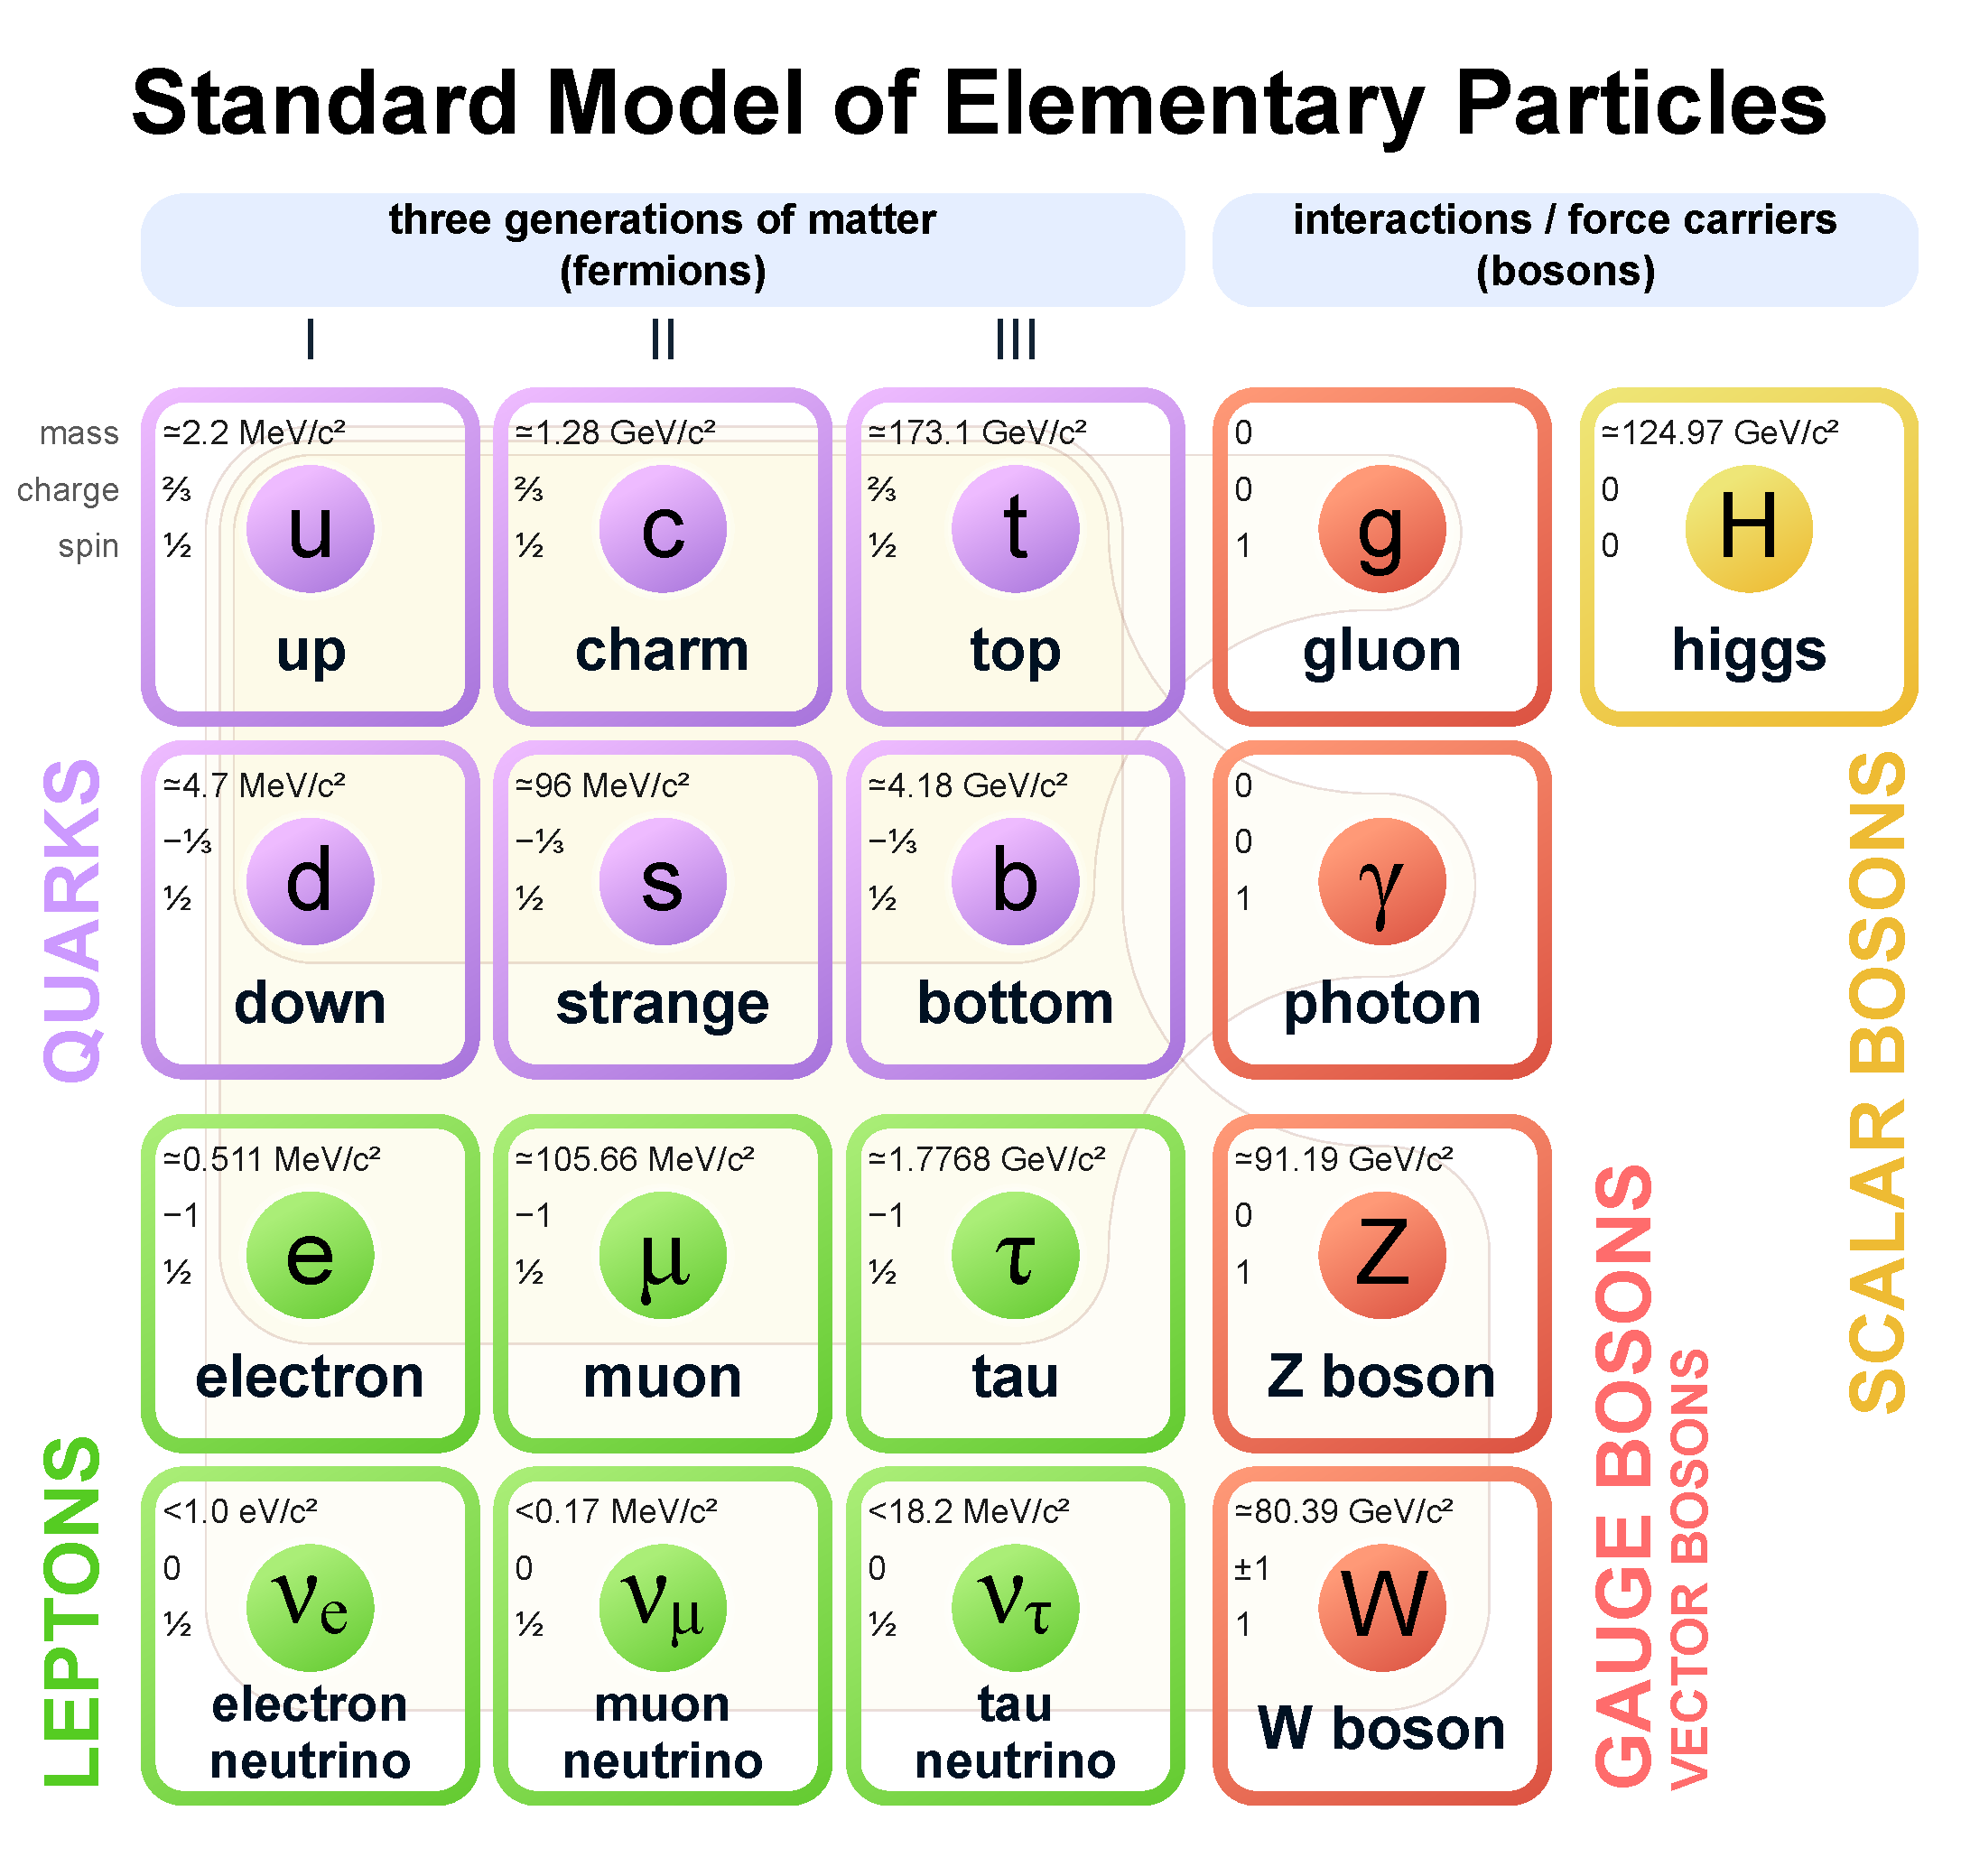
\includegraphics[width=\textwidth]{figures/Standard_Model_of_Elementary_Particles.pdf}
		\caption{\label{intro-fig:standard model}Diagram of the Standard Model of particle physics, as it currently stands. From \cite{cush_standard_2019}}
	\end{centering}
	\end{figure} 
	The 17 known particles are organized in a framework called the Standard Model of particle physics \cite{larkoski_elementary_2019-1,schwartz_quantum_2014}, displayed in schematic form in Fig.~\ref{intro-fig:standard model}.

	There are 12 particles, called \textbf{fermions}, which are the fundamental components of matter. These in turn are subdivided into \textbf{quarks} and \textbf{leptons}. Quarks, with names such as `up,' `down,' and `strange,' combine in turn to form \textbf{hadrons} --- among the hadrons are familiar composite particles like protons and neutrons. 

	The remaining 5 particles, called \textbf{bosons}, mediate interactions between particles. Four of these are responsible for three of the forces of nature: the \textbf{gluon} is responsible for the strong force; the \textbf{photon} is responsible for the electromagnetic force; and the \textbf{$W$ and $Z$ bosons} are responsible for the weak force. In terms of familiar phenomena, the strong force is what binds together the nuclei of atoms; the electromagnetic force is what makes possible most of chemistry, electronics, and modern technology; and the weak force is responsible for the decay of unstable nuclei and particles. The final boson, the \textbf{Higgs boson}, is responsible for giving mass to most of the fundamental particles, and in a technical sense is the keystone which holds the Standard Model together.

	In the Standard Model, each fermion is beholden to some subset of these bosons. The neutrinos experience the weak force and so interact via the $W$ and $Z$ bosons. The electron, muon, and tau experience the weak force as well, but they can also interact electromagnetically through exchange of photons. The quarks experience all of the fundamental forces, and can interact via any of the force-carrying bosons. It is the interaction of quarks and gluons through the strong force which will occupy most of this thesis.


\subsection{(In)completeness of the Standard Model}
	The Standard Model is a remarkable theory. It explains many observed phenomenon with unparalleled accuracy --- in fact, the Standard Model explanation of electromagnetism, called quantum electrodynamics, is the most precise physical theory ever constructed, making predictions that agree to less than 1 part per billion \cite{larkoski_elementary_2019-1}. Experiment after experiment has confirmed predictions of the Standard Model, and in this sense it is a triumph of 20th-century physics.

	In the present century, however, the strength of the theory is a significant problem in the field --- for we know that the Standard Model is incomplete. While the theory is successful at describing small-scale physics, it is not nearly as successful on a cosmic scale: it has been observed that 84.4\% of all matter in the universe is unknown to us and invisible except by gravitational signatures \cite{particle_data_group_review_2020}. We would like to understand the composition of this so-called `dark matter.' There are also more earthly hints that the Standard Model is incomplete. Among these, one of the most famous is the existence of neutrino masses. While the Standard Model describes neutrinos as massless particles, the Super-Kamiokande experiment discovered evidence in 1998 that neutrinos have a (tiny) non-zero mass \cite{super-kamiokande_collaboration_evidence_1998} --- these observations have since been verified by numerous other experiments \cite{particle_data_group_review_2020}. Finally, there are aesthetic considerations. The Standard Model, as it currently stands, has a multitude of parameters (e.g., the masses of different particles) that currently have no basis in the theory; they must be supplied externally. If possible, we would like to be able to predict these parameters eventually.\footnote{One can hardly say they understand something if, when asked why a particular detail is just so, their response is no more sophisticated than ``That's just the way it is.''}

	Thus, the Standard Model is incomplete. What can we do about that? There are two primary approaches to finding a solution:
	\begin{enumerate}
		\item \textbf{Searches for new particles:} one strategy is to design experiments that attempt to generate and detect new, previously unobserved particles. This is a well-worn technique in particle physics, responsible for many of the advances in the field over the last 20th century. Famous examples of new-particle discoveries include the $J/\psi$ in 1974 \cite{aubert_experimental_1974,augustin_discovery_1974}, the discovery of the top quark in 1995 \cite{d0_collaboration_observation_1995,cdf_collaboration_observation_1995}, and the discovery of the Higgs boson in 2012 \cite{atlas_collaboration_observation_2012,cms_collaboration_observation_2012}. Historically, whenever new experimental frontiers have been explored, new discoveries have followed, and with them, new understanding. This is not, of course, a guarantee that such will continue in the future.\footnote{Past performance is not a guarantee of future returns.} Nevertheless, it is the underlying (if simplified) philosophy for many new particle searches at modern experiments.

		\item \textbf{Precision measurements of Standard Model parameters:} another, complementary strategy is to measure parameters of the Standard Model very precisely and then compare these measurements to theoretical predictions. These parameters could be anything from particle masses, to the strength of coupling constants, to the probability of a particular event after a particular interaction. If a discrepancy emerges, then that is a clue about where to consider modifying the Standard Model. Note, however, that to put a precise experimental measurement into a proper context, it is necessary to have at hand a precise theory. If we could measure, say, the mass of the muon\footnote{Compared to the state of the art, this would be an outrageously precise measurement. The mass of the muon is currently accepted to be \SI{105.6583745(24)}{\mega\electronvolt} \cite{particle_data_group_review_2020}, which is a precision of approximately 1 part in $10^{8}$.} to 1 part in $10^{20}$, it would do us no good if the theoretical prediction were only confident to 1 part in $10^5$. Theory and experiment must both be sufficiently advanced to take full advantage of a precise measurement.
	\end{enumerate}

	This thesis is situated firmly in the latter camp. We will be interested in precision theoretical predictions of a particular observable, called the `groomed heavy hemisphere mass mass,' measured in high-energy electron-positron collisions. More will be said on this topic in due time.


\subsection{Collider experiments}
	Although this thesis is theoretical in nature, it will be helpful to have some familiarity with the experiments whose outcomes we would like to predict. There is an enormous variety of experiments in particle physics, and it would be neither feasible nor helpful to discuss them all here. Instead, let us examine the two modern experiments most pertinent for our study to come. These experiments are called ATLAS (\textbf{A} large \textbf{T}oroidal \textbf{L}HC \textbf{A}pparatu\textbf{S}) and CMS (\textbf{C}ompact \textbf{M}uon \textbf{S}olenoid).\footnote{Acronyms in particle physics get very unwieldy very quickly. But look how much fun they are!} 

	Both of these are located at the Large Hadron Collider (LHC) at CERN in Geneva, Switzerland. The name of this collider is appropriate. Beams of protons are accelerated to around 99.9998\% of the speed of light using a circular ring approximately \SI{27}{\kilo\metre} in circumference.\footnote{The ring straddles the French-Swiss border.} Two beams circulate in the collider at a time, one traveling clockwise, the other counterclockwise. These beams are then maneuvered into collisions at four points around the ring, each located in the center of a massive, purpose-built experiment (in addition to ATLAS and CMS, there are two other experiments, called ALICE and LHCb). That is when the magic begins --- the collision of these protons at high energy produces, through fundamental interactions, a huge variety of particles. By observing these particles, we hope to learn something about the interactions that brought them into being.

	\begin{figure}
	\begin{center}
		\includegraphics[width=\textwidth]{figures/atlas_high_res.jpg}
		\caption{\label{intro-fig:atlas diagram}Schematic of the ATLAS experiment. For a sense of scale, note the people depicted along the bottom. Image from CERN \cite{cern_ac_layout_1998}}
	\end{center}
	\end{figure}

	ATLAS and CMS are designed as multi-purpose experiments which detect all the products of the proton-proton collisions (or at least, they try to detect them). A schematic of the ATLAS detector is displayed in Fig.~\ref{intro-fig:atlas diagram}, and a schematic of CMS is displayed in Fig.~\ref{intro-fig:cms diagram}. These detectors are built in layers surrounding the \textbf{interaction point}, with each layer serving a dedicated purpose. These layers can be summarized as follows \cite{larkoski_elementary_2019-1}:
	\begin{enumerate}
		\item In the center of each detector is the \textbf{beam pipe}. This is where collisions take place.

		\item Immediately surrounding the beam pipe is a \textbf{tracking system}. The objective of this system is to track particles as they fly away from the interaction point. From these tracks, we can glean information about the energy, charge, and type of the particles.

		\item Outside the tracking system is a \textbf{calorimetry system}. These are divided into two parts, the \textbf{electromagnetic calorimeter} and the \textbf{hadronic calorimeter}. The calorimetry system records information about the energy of particles. It works by absorbing this energy directly. The electromagnetic calorimeter is designed to most efficiently absorb particles which interact primarily through electromagnetism: electrons, photons, and the like. The hadronic calorimeter is designed to absorb hadrons like protons and neutrons.

		\item High-energy muons often escape all inner layers of the detector. Their properties are measured using \textbf{muon detectors} which line the detector's exterior.
	\end{enumerate}

	\begin{figure}
	\begin{center}
		\includegraphics[width=\textwidth]{figures/cms_160312_02.pdf}
		\caption{\label{intro-fig:cms diagram}Schematic of the CMS experiment. Note the person on the far right for scale. Image from \cite{sakuma_detector_2014}}
	\end{center}
	\end{figure}

	Using these systems, ATLAS and CMS are able to measure the results of more than a billion collision events per second, though the data is rapidly processed through a \textbf{triggering} system to reduce stored data rates to the \si{\kilo\hertz} level. \cite{atlas_outreach_atlas_2012,atlas_collaboration_performance_2017}. This data gets stored and processed at data centers distributed globally.\footnote{The scale of ATLAS and CMS is absolutely mind-boggling.} Typical searches and measurements at these experiments then look for statistical signatures of interesting physics. This could be anything from an unexpected excess of events in a particular region of phase space (for a particle search) to the probability distribution of observing particular values of particle parameters (for Standard Model measurements). 


\section{Thesis goals}
	The objectives of this thesis can be divided into two categories: scientific and pedagogical. It will be necessary to properly balance the two. Our scientific focus will be rather technical, and too much emphasis on this would cloud the narrative and make it difficult to learn from the work. The other side of this coin is that, to achieve the pedagogical goals of the thesis, we will have to complete only a partial calculation. This is not a complete loss --- what we achieve will be meaningful in its own right, and we will not have to suffer unnecessary tedium. Nevertheless, I warn the reader in advance that the story will be left incomplete.

	But enough digression --- what are the goals?

\subsection{Scientific}
	The primary scientific objective of the thesis will be to complete an all-orders calculation of the distribution of groomed heavy hemisphere mass in $e^+ e^- \to \text{jets}$ events, in the limit that the jet mass is approximately equal to the grooming cutoff. There are several moving parts here:
	\begin{enumerate}
		\item \textbf{$e^+ e^- \to \text{jets}$ events:} We are going to consider collider events in which electron and positrons annihilate to produce quarks and gluons. At high energies, because of the nature of the strong force, quarks and gluons manifest themselves in a detector as \textbf{jets}, or collimated sprays of hadronic particles. Note that these are not the type of collision events observed at the LHC, which is a proton-proton collider. Electron-positron annihilation is much easier to handle theoretically, and it turns out that we can generalize our results to $pp$ collisions without much difficulty.

		\item \textbf{Heavy hemisphere mass:} We are interested in an observable called heavy hemisphere mass. To compute heavy hemisphere mass, one can divide a collision event into two hemispheres, measure the mass of both hemispheres, and then take the greater of the two masses.

		\item \textbf{Groomed:} When measuring an observable like jet mass, modern experiments like ATLAS and CMS must take into account significant amounts of background radiation from simultaneous events in the detector. One common technique is to perform `jet grooming,' in which undesirable radiation is algorithmically removed from a jet. We will consider a particular grooming algorithm called the Modified Mass Drop Tagger (mMDT) \cite{dasgupta_towards_2013}, in which radiation with energy below some threshold is ignored. Such grooming can significantly alter the distribution of an observable, and it has important experimental and theoretical advantages. Understanding the effect of grooming on observables like jet mass is an active area of research.

		\item \textbf{The limit:} Jets are a phenomenon of the strong force, and the theory of the strong force is rather unwieldy. It is therefore difficult to accurately predict an entire observable distribution with only one calculation. While the distribution of groomed heavy hemisphere mass is well understood in the low-mass limit \cite{kardos_groomed_2020,kardos_two-_2020,frye_factorization_2016} and in the high-mass regime \cite{kardos_soft-drop_2018}, little study has been performed in the regime where the mass is approximately equal to the mMDT energy cutoff. Nevertheless, interesting physics occurs in this region --- whereas events throughout the distribution all rely on the production of two back-to-back quarks, this region is the one in which a third (gluon) emission just begins to be resolved above the grooming threshold. Thus, this region is our focus.

		\item \textbf{Calculation:} Just as we must perform calculations in particular limits to work with the strong force, so we must also perform calculations perturbatively, as a series expansion in the strong coupling constant $\alpha_s$. That is, if we want to compute an observable $\omega$, it is not usually feasible\footnote{At least with current theoretical techniques.} to do so with perfect precision. Instead, we can expand $\omega$ in $\alpha_s$,
		\begin{equation}
			\omega(\alpha_s) = \omega_0 + \omega_1 \alpha_s + \omega_2 \alpha_s^2 + \dots = \sum_{n = 0}^\infty \omega_n \alpha_s^n.
		\end{equation}
		Then, to compute $\omega$ to a particular desired accuracy, we can simply compute the coefficients $\omega_i$ up to a particular order in $\alpha_s$. Unfortunately, $\alpha_s$ is not a particularly small quantity, taking a value of order $0.1$.\footnote{The strong coupling constant is not actually a constant\dots it changes with the energy of observation. This process is called the \textbf{running} of the strong coupling \cite{larkoski_elementary_2019-1}. At the mass of the $Z$ boson, $\alpha_s(m_Z) = 0.1179(10)$ \cite{particle_data_group_review_2020}.} This means it often takes several terms to obtain a reasonable degree of accuracy.

		\item \textbf{All-orders:} That said, we are aiming to achieve an all-orders calculation of the groomed heavy hemisphere mass. This does \textit{not} mean that we will determine the distribution to infinite precision (i.e., infinite order in $\alpha_s$). Instead, it means that we will derive an expression which can be used to push to \textit{arbitrary accuracy} in $\alpha_s$, given the proper accuracy of inputs (and the proper degree of mathematical sophistication). Thus, by an `all-orders calculation,' we mean that we will develop a \textit{framework} for achieving precision results. The term `all-orders' also refers to the fact that our calculation will account for the influence of large logarithms at every order in $\alpha_s$ through the process of resummation.
	\end{enumerate}
	A more complete development of these foundational concepts will be provided in Chapter \ref{chap:technical}.


\subsection{Pedagogical}
	The primary pedagogical goal of this thesis is to understand the inner workings of a particular class of precision calculations in modern high-energy physics. The scientific objectives described above require a set of advanced theoretical tools which are interesting in their own right, but difficult to understand except through examples and context. Such tools include:
	\begin{enumerate}
		\item \textbf{Dimensional regularization:} There will be times when we must evaluate an integral which diverges when computed in the usual 4 dimensions (3 spatial dimensions and one temporal). We will get around this problem by performing such calculations in $d = 4 - 2\epsilon$ dimensions for some small $\epsilon$ \cite{schwartz_quantum_2014}. The result will still diverge if we send $\epsilon \to 0$, but operating in this way will allow us to see the divergences explicitly, and cancel them as appropriate.

		\item \textbf{Resummation:} A na\"ive series expansion of the distribution which we want to compute is plagued by corrections that take the form of logarithms of ratios of differing energy scales (e.g., the energy scale of a jet versus the energy scale of background radiation). When these scales are sufficiently different, the logarithm of their ratio becomes very large. Resummation is the process of getting a theoretical handle on these logarithmic corrections \cite{larkoski_elementary_2019-1}. The primary thrust of this thesis can be viewed, in a sense, as one large resummation calculation.

		\item \textbf{Soft and collinear effective theory (SCET):} Quantum field theory (QFT) is a remarkable description of the (subatomic) universe, but for our purposes it is too much machinery. Instead of using the full theory, we will make use of a low-energy effective theory called `soft and collinear effective theory' (SCET). SCET is essentially a limiting case of full QFT, useful in the regime which we will occupy ourselves. As a simpler theory, SCET has some useful properties that we will exploit.
	\end{enumerate}


\section{Technical and notational conventions}
	Before we embark, we must lay some mathematical ground rules. First, we hold Planck's constant and the speed of light to be equal to unity: $\hbar = c = 1$. It turns out that non-unity values of these quantities are, for our purposes, redundant; when converting a given quantity back to SI units, the appropriate factors of $c$ and $\hbar$ can be intuited from context. The result is that all quantities will be measured in units of energy. Physics where we will be working is at the \si{\giga\electronvolt} scale and higher. Therefore, to a high degree of accuracy, we will assume all particles to be massless.

	Unless otherwise stated (and we \textit{will} eventually state otherwise), we will work in $4$ dimensions, comprising the usual three spatial dimensions and one temporal dimension. Vectors in $4$ dimensions (called four-vectors) are denoted by a Greek-letter index and take the form
	\begin{equation}
		p^\mu = (p^0, p^1, p^2, p^3).
	\end{equation}
	The $0$-th component of a four-vector is its `time' (or equivalent) component, and the others are the `spatial' (or equivalent) components. Thus, for example, a four-vector representing position would be
	\begin{equation}
		x^\mu = (t, x, y, z),
	\end{equation}
	while a four-momentum has the components
	\begin{equation}
		p^\mu = (E, p_x, p_y, p_z)
	\end{equation}
	with energy taking the place of time. It is sometimes convenient to refer to lower-dimensional pieces of a four-vector (usually two or three of the spatial components). When doing so, we will denote the sub-vector using a bold-face letter:
	\begin{equation}
		p^\mu = (E, \vb{p}), \quad \vb{p} = (p_x, p_y, p_z).
	\end{equation}

	As is standard in high-energy physics, we will neglect the effects of gravity and assume we are working in a flat space-time. When combining four-vectors, we will therefore use the `mostly minus' metric\footnote{Also known as the `West Coast' metric, among other names. The `East Coast' metric takes the opposite sign convention. Our convention here is clearly the correct one, as it results in naturally positive masses.}
	\begin{equation}
		\eta^{\mu \nu} = \begin{pmatrix}
			1 & 0 & 0 & 0 \\
			0 & -1 & 0 & 0 \\
			0 & 0 & -1 & 0 \\
			0 & 0 & 0 & -1
		\end{pmatrix}.
	\end{equation}
	We will also employ the Einstein summation notation, in which one sums over repeated indices in an expression (known as `contracting' the index). Hence, for $p^\mu = (p^0, \vb{p})$ and $k_\mu = (k_0, \vb{k})$, we have
	\begin{equation}
		k_\mu p^\mu = k_0 p^0 + k_1 p^1 + k_2 p^2 + k_3 p^3.
	\end{equation}

	With our choice of metric, there is little mechanical difference between a contravariant and a covariant four-vector; one picks up a formal minus sign in the spatial components, but that is all. We will, therefore, not distinguish between the two, and we will interchange upper and lower indices freely, bearing in mind that contracting an index negates the spatial terms of the sum. Hence, for $p^\mu = (p^0, \vb{p})$ and $k^\mu = (k^0, \vb{k})$, we will write\footnote{Sorry, Joel.}
	\begin{equation}
		k^\mu p_\mu = k_\mu p^\mu = k^\mu p^\mu = k_\mu p_\mu = k^0 p^0 - \vb{k} \cdot \vb{p}.
	\end{equation}
	The final term is the standard dot product between the three-vectors. This choice enables us to abuse notation in a convenient manner: we will often drop the Greek sub/superscript on four-vectors, and use the standard notation of linear algebra to indicate their contraction:
	\begin{equation}
		k \cdot p = k^0 p^0 - \vb{k}\cdot\vb{p}.
	\end{equation}

	Let us end with a reminder about the connection between these four-vectors and the physical world. Suppose a particle has a momentum four-vector $p^\mu$. Transforming our frame of reference to the particle's rest frame, we could write $p^\mu = (E, 0, 0, 0)$, where $E$ is the particle's energy. But then, recalling the famous relation $E = mc^2 = m$ (since we set $c = 1$), we have
	\begin{equation}
		p^2 = p \cdot p = E^2 = m^2.
	\end{equation}
	Thus, the square of a particle's four-momentum yields its squared mass. Recall now that we are assuming all particles to be massless; therefore, for any `on-shell' particle (that is, a particle that could exist on its own and not just in some quantum fluctuation), we see that $p^2 = 0$, and also that $E^2 = \vb{p} \cdot \vb{p}$.\footnote{This is not strictly an accurate proof of these properties, since massless particles move at the speed of light and one cannot boost into a light-like reference frame using Lorentz transformations. But the spirit of the argument is right, and the result is the same regardless.} This will greatly simplify our calculations later on.

	With these details out of the way, let us proceed.

% \ifstandalone
% \bibliographystyle{../bsts/myJHEP} 
% \bibliography{../jet_substructure}
% \fi
\end{document}
